\documentclass{article}
\usepackage[english,ngerman]{babel}
\usepackage{fullpage}
%\documentclass[9pt,lineno]{elife}
\usepackage{graphicx}
\graphicspath{{./figures/}}

\begin{document}
\begin{figure}[htp]
  \begin{center}
  \includegraphics[width=\textwidth]{Fig1.pdf}
   \end{center}
\end{figure}
\newpage
\begin{figure}[htp]
  \begin{center}
  \includegraphics[width=\textwidth]{Fig2.pdf}
   \end{center}
\end{figure}
\newpage{}
\begin{figure}[htp]
  \begin{center}
  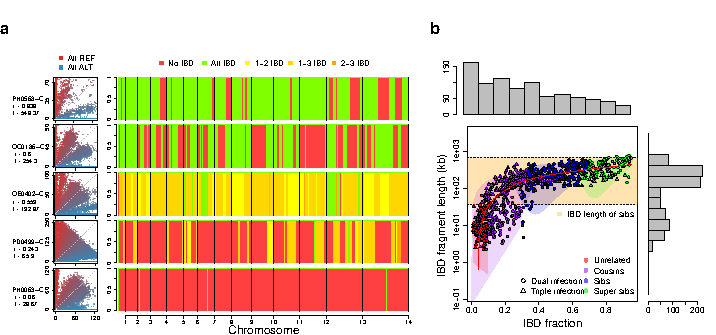
\includegraphics[width=\textwidth]{Fig3.pdf}
   \end{center}
\end{figure}
\newpage{}
\begin{figure}[htp]
  \begin{center}
  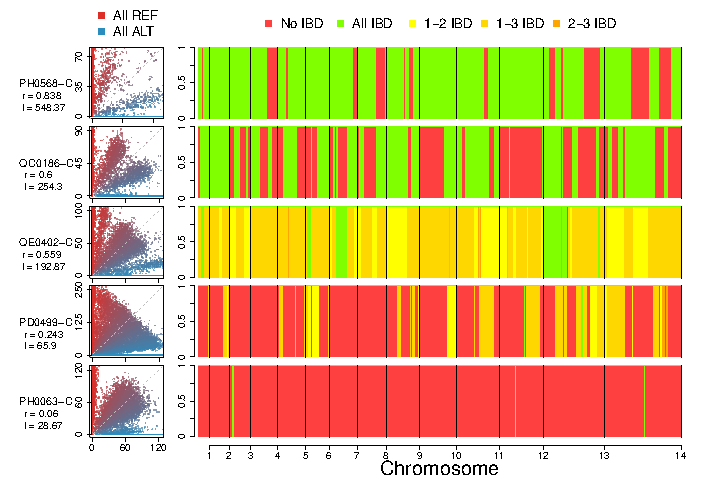
\includegraphics[width=\textwidth]{Fig4.pdf}
   \end{center}
\end{figure}
\newpage{}
\begin{figure}[htp]
  \begin{center}
  \includegraphics[width=\textwidth]{Fig5.pdf}
   \end{center}
\end{figure}
\newpage{}
\begin{figure}[htp]
  \begin{center}
  \includegraphics[width=\textwidth]{Fig6.pdf}
   \end{center}
\end{figure}

\end{document}
